\documentclass{article}
\usepackage{graphicx}
\graphicspath{ {../diagram/} }
\usepackage[margin=2cm]{geometry}
\usepackage{enumitem}
\usepackage{caption}
\usepackage{subcaption}
\usepackage{amsmath}
\usepackage{booktabs}

\title{DSP in VLSI \\ Homework 4 - CORDIC}
\author{Jen-Tse Chen}
\date{April 2026}

\begin{document}
\maketitle

\begin{enumerate}

    \item (Step 1) Please draw the figure showing $S(N)$ versus $N$ for $N = 1\ldots 30$. (5\%)

    Figure~\ref{fig:scaling_factor} shows the CORDIC scaling factor $S(N) = \prod_{i=0}^{N-1} \frac{1}{\sqrt{1+2^{-2i}}}$ versus the number of micro-rotations $N$. The factor decreases rapidly and converges to approximately $0.6073$ by $N \approx 5$, remaining constant thereafter.

    \begin{figure}[htbp]
        \centering
        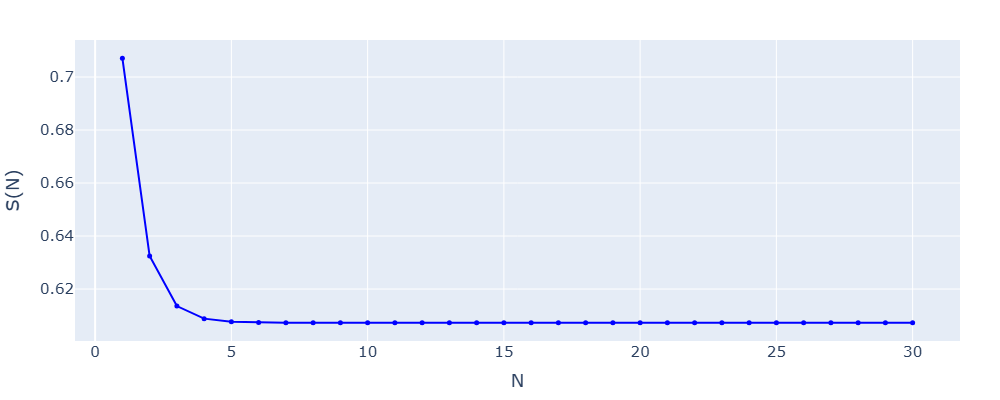
\includegraphics[width=1.0\textwidth]{../diagram/Q1/scaling_factor.png}
        \caption{CORDIC scaling factor $S(N)$ versus $N$}
        \label{fig:scaling_factor}
    \end{figure}

    % \newpage
    \item (Step 2) Draw the figure of average absolute error versus fractional wordlength (10\%) to show how you determine the setting of word-length of the fractional part. Write down the integer word-length of $X(i)$ and $Y(i)$ that you use all the stages. Please explain it. (5\%)

    Figure~\ref{fig:avg_error_vs_wordlength} plots the average absolute phase error against the fractional wordlength $w$ with $N = 30$ micro-rotations.
    The error decreases monotonically and falls below the $2^{-9}$ criterion at $w = 9$, after which further increase yields negligible improvement for the phase function.
    However, the magnitude function analysis in Step~4 shows that 9 fractional bits cause accumulated truncation error to violate the 0.1\% magnitude criterion across most micro-rotation counts.
    Therefore, the fractional wordlength of the $X$ and $Y$ datapath is set to $w = 12$ bits to satisfy both the phase and magnitude requirements.

    Each CORDIC micro-rotation is a pseudo-rotation that does not preserve the vector magnitude; the amplitude grows by a factor of $1/S(N)$.
    For unit-circle inputs ($\sqrt{X_0^2 + Y_0^2} = 1$) the maximum value reached by either register throughout all $N$ stages is bounded by
    \[
        \max_i \sqrt{X(i)^2 + Y(i)^2} \;=\; \frac{1}{S(N)} \;\approx\; 1.647 \;<\; 2^1.
    \]
    Since the pseudo-magnitude never reaches $2$, one integer bit suffices for all stages.
    Combined with the sign bit, the complete word format is 1 sign $+$ 1 integer $+$ 12 fractional $= 14$ bits.

    \begin{figure}[htbp]
        \centering
        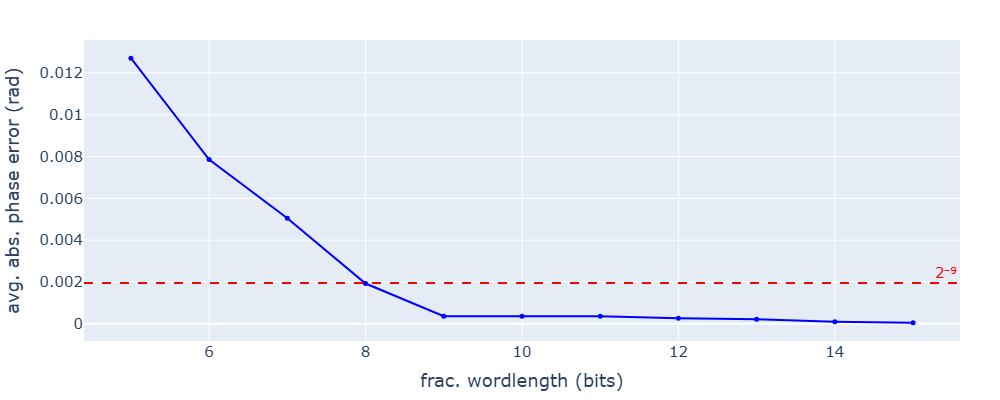
\includegraphics[width=1.0\textwidth]{../diagram/Q2/phase_error_vs_wordlength.png}
        \caption{Average absolute phase error versus fractional wordlength $w$ of $X(i)$ and $Y(i)$ ($N = 30$, floating-point $\theta$)}
        \label{fig:avg_error_vs_wordlength}
    \end{figure}

    \newpage
    \item (Step 3) Please draw a figure to denote the average phase errors of 10 quantized input pairs $(X, Y)$ versus different numbers of micro-rotations $S$ (10\%) and draw a figure to show the resulted phase errors of 10 quantized input pairs versus the word-length of quantized elementary angles (10\%). Explain your selection to satisfy the averaged error criterion of $2^{-9}$ radian. Also list a table of the elementary angles (both in floating-point representation and binary fixed-point representation). (5\%)

    Figure~\ref{fig:error_vs_S} shows the average absolute phase error versus the number of micro-rotations $N$, with the $X$ and $Y$ fractional wordlength fixed at 12 bits.
    The error decreases as $N$ increases and first falls below the $2^{-9}$ criterion at $N = 10$.
    Therefore, the number of micro-rotations is set to $N = 10$.

    Figure~\ref{fig:error_vs_angle_wordlength} shows the average absolute phase error versus the fractional wordlength of the quantized elementary angles, with $N = 10$ micro-rotations and $X$ and $Y$ fractional wordlength fixed at 12 bits.
    The error decreases with increasing wordlength, meets the $2^{-9}$ criterion at 10 bits, and saturates beyond that point because the dominant error source shifts to the $X$ and $Y$ quantization.
    Therefore, the fractional wordlength of the elementary angle LUT is set to 10 bits.

    \begin{figure}[htbp]
        \centering
        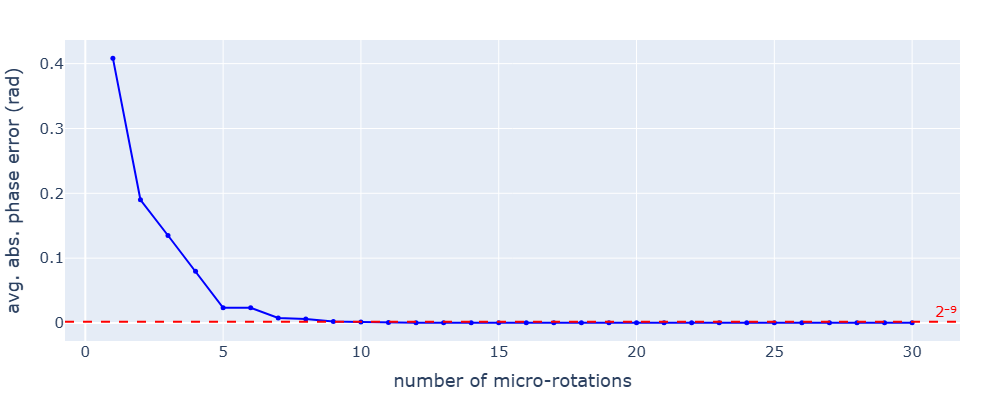
\includegraphics[width=1.0\textwidth]{../diagram/Q3/phase_error_vs_micro_rotation.png}
        \caption{Average absolute phase error versus number of micro-rotations $N$ (fractional wordlength of $X$ and $Y$ = 12 bits, floating-point elementary angles)}
        \label{fig:error_vs_S}
    \end{figure}

    \begin{figure}[htbp]
        \centering
        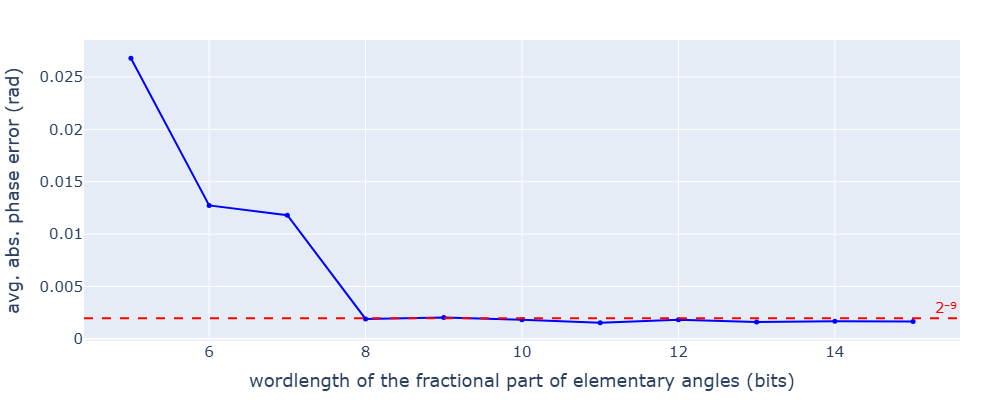
\includegraphics[width=1.0\textwidth]{../diagram/Q3/phase_error_vs_theta_wordlength.png}
        \caption{Average absolute phase error versus fractional wordlength of quantized elementary angles ($N = 10$, fractional wordlength of $X$ and $Y$ = 12 bits)}
        \label{fig:error_vs_angle_wordlength}
    \end{figure}

    The 10 elementary angles used in the CORDIC micro-rotations are listed in Table~\ref{tab:elementary_angles}.

    \begin{table}[htbp]
    \centering
    \begin{tabular}{ccc}
    \toprule
    $i$ & $\theta_e(i) = \arctan(2^{-i})$ (rad) & Binary fixed-point (10 frac.~bits) \\
    \midrule
        0 & 0.7853981634 & \texttt{0.1100100100} \\
        1 & 0.4636476090 & \texttt{0.0111011011} \\
        2 & 0.2449786631 & \texttt{0.0011111011} \\
        3 & 0.1243549945 & \texttt{0.0001111111} \\
        4 & 0.0624188100 & \texttt{0.0001000000} \\
        5 & 0.0312398334 & \texttt{0.0000100000} \\
        6 & 0.0156237286 & \texttt{0.0000010000} \\
        7 & 0.0078123411 & \texttt{0.0000001000} \\
        8 & 0.0039062301 & \texttt{0.0000000100} \\
        9 & 0.0019531225 & \texttt{0.0000000010} \\
    \bottomrule
    \end{tabular}
    \caption{Elementary angles $\theta_e(i)$ in floating-point and 10-bit fixed-point binary representation}
    \label{tab:elementary_angles}
\end{table}


    % \newpage
    \item (Step 4) Please show how you decide the number of micro-rotations for the magnitude function with error tolerance of 0.1\%. (10\%)

    Figure~\ref{fig:error_vs_N_magnitude} shows the average relative magnitude error versus the number of micro-rotations $N$, with the $X$ and $Y$ fractional wordlength set to 12 bits (as determined in Step~2).
    The 0.1\% criterion is satisfied for $N \geq 5$.
    Combining with the conclusion from Step~3, the number of micro-rotations is kept at $N = 10$.

    \begin{figure}[htbp]
        \centering
        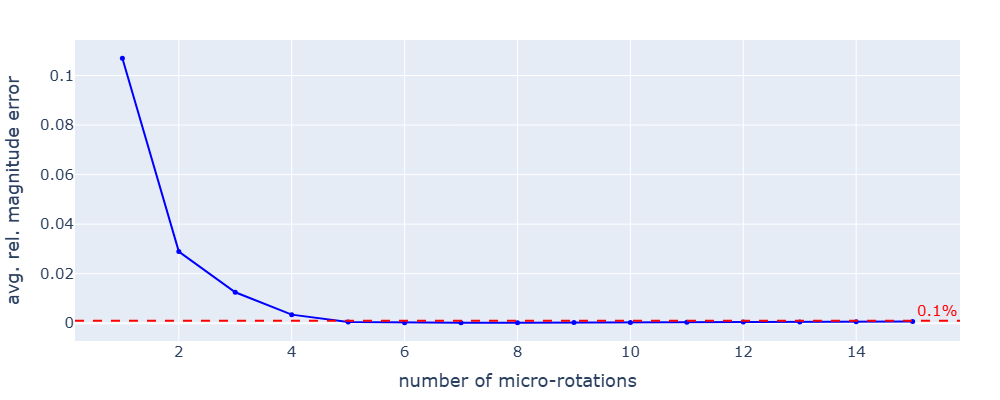
\includegraphics[width=1.0\textwidth]{../diagram/Q4/error_vs_N_magnitude.png}
        \caption{Average relative magnitude error versus number of micro-rotations $N$ (fractional wordlength of $X$ and $Y$ = 12 bits)}
        \label{fig:error_vs_N_magnitude}
    \end{figure}

    % \newpage
    \item (Step 5) Write a program to show the setting of fractional wordlength of CSD versus error. Draw the figure. (10\%) Depict your design for the shift-and-add block according to your CSD representation. How many adders do you use? (10\%)

    Figure~\ref{fig:csd_error_vs_wordlength} shows the average relative magnitude error versus the fractional wordlength of the CSD representation of $S(N)$, with $N = 10$ and $X$ and $Y$ fractional wordlength fixed at 12 bits.
    The 0.1\% criterion is first satisfied at a fractional wordlength of 9 bits.
    Therefore, the CSD scaling factor is quantised to 9 fractional bits.

    At 9 fractional bits, $S(10) \approx (-2^{0}-2^{3}+2^{6}+2^{8})/512$. With 4 non-zero CSD digits the multiplication requires 3 adders.

    \begin{figure}[htbp]
        \centering
        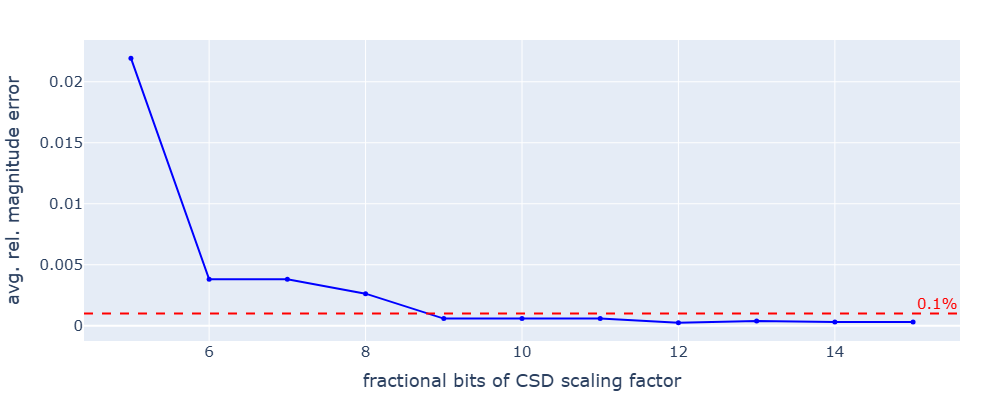
\includegraphics[width=1.0\textwidth]{../diagram/Q5/error_vs_csd_frac_bits.png}
        \caption{Average relative magnitude error versus fractional wordlength of the CSD scaling factor $S(10)$ ($N = 10$, fractional wordlength of $X$ and $Y$ = 12 bits)}
        \label{fig:csd_error_vs_wordlength}
    \end{figure}

    \begin{figure}[htbp]
        \centering
        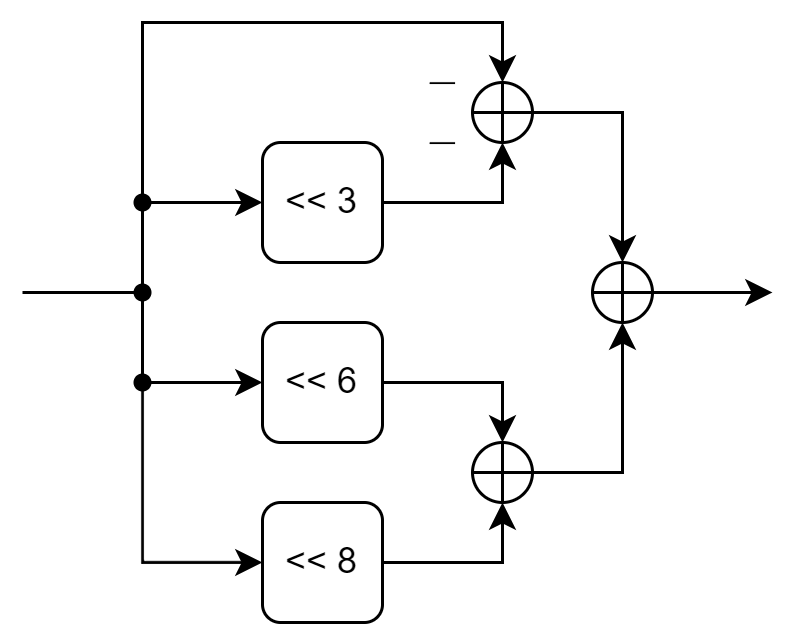
\includegraphics[width=0.35\textwidth]{../diagram/Q5/scaling_factor_mult.png}
        \caption{Shift-and-add block diagram for the CSD scaling factor $S(10)$}
        \label{fig:scaling_factor_mult}
    \end{figure}

    \newpage
    \item (Step 6) Depict your design of the initial stage. Mark the word-length in the block diagram. (10\%)

    Figure~\ref{fig:initial_stage} shows the block diagram of the initial stage. The initial stage maps the complex input into the right half plane before the CORDIC iterations begin; the offset shifts back to the original quadrant after the CORDIC iterations.

    \begin{figure}[htbp]
        \centering
        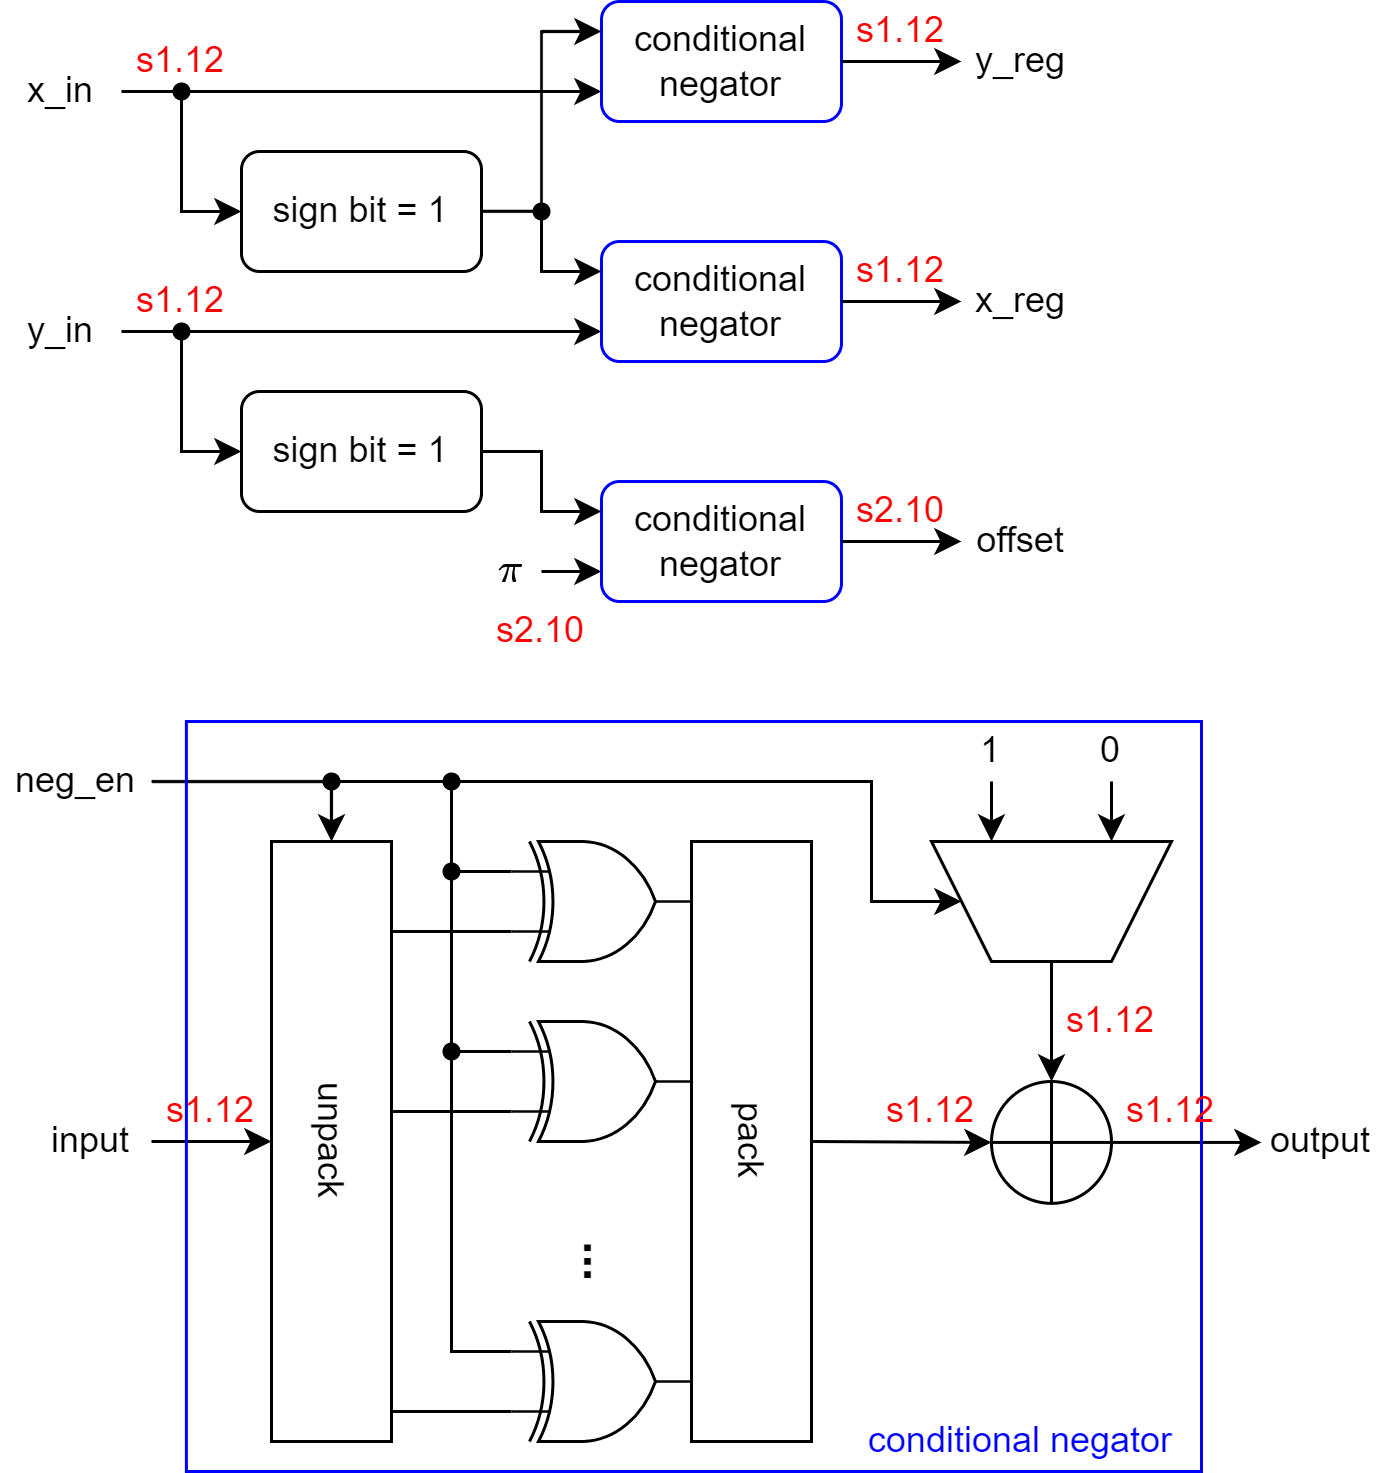
\includegraphics[width=0.6\textwidth]{../diagram/Q6/init_stage.png}
        \caption{Block diagram of the initial stage with word-lengths marked}
        \label{fig:initial_stage}
    \end{figure}

    \newpage
    \item (Step 6) Implement your design with only DFFs inserted at the inputs and outputs. Show the timing diagram of behavior simulation for four inputs. (15\%) Compare the results with the arctangent function and draw the error versus index $m$ to show that your implementation meets the precision requirements of error less than $2^{-9}$. (10\%)

    \begin{figure}[htbp]
        \centering
        % \includegraphics[width=0.75\textwidth]{../diagram/Q7/timing_behav.png}
        \caption{Timing diagram of behavior simulation for four inputs}
        \label{fig:timing_behav}
    \end{figure}

    \begin{figure}[htbp]
        \centering
        % \includegraphics[width=1.0\textwidth]{../diagram/Q7/error_vs_m_behav.png}
        \caption{Phase error versus index $m$ for iterative architecture (behavior simulation)}
        \label{fig:error_vs_m_behav}
    \end{figure}

    \newpage
    \item (Step 7) Draw the block diagram of your $\frac{S}{2}$-unfolding architecture. (10\%) Show the timing diagram of behavior and post-synthesis simulation with correct setting of clock period and 10 inputs. (30\%) Verified the error between the post-synthesis results and the floating-point arctangent results. Draw the error versus index $m$. (10\%)

    \begin{figure}[htbp]
        \centering
        % \includegraphics[width=0.75\textwidth]{../diagram/Q8/unfolding_arch.png}
        \caption{Block diagram of the $\frac{S}{2}$-unfolding architecture}
        \label{fig:unfolding_arch}
    \end{figure}

    \begin{figure}[htbp]
        \centering
        % \includegraphics[width=0.75\textwidth]{../diagram/Q8/timing_behav_10inputs.png}
        \caption{Timing diagram of behavior simulation with 10 inputs}
        \label{fig:timing_behav_10inputs}
    \end{figure}

    \begin{figure}[htbp]
        \centering
        % \includegraphics[width=0.75\textwidth]{../diagram/Q8/timing_postsyn_10inputs.png}
        \caption{Timing diagram of post-synthesis simulation with 10 inputs}
        \label{fig:timing_postsyn_10inputs}
    \end{figure}

    \begin{figure}[htbp]
        \centering
        % \includegraphics[width=1.0\textwidth]{../diagram/Q8/error_vs_m_postsyn.png}
        \caption{Phase error versus index $m$ for $\frac{S}{2}$-unfolding architecture (post-synthesis)}
        \label{fig:error_vs_m_postsyn}
    \end{figure}

    \newpage
    \item (Step 8) Report and compare the area before and after unfolding. (10\%)

    \newpage
    \item (Step 9) Draw the shift-and-add module for the scaling factor (5\%). Connect the shift-and-add module to your micro-rotation module, and calculate the magnitude function. Show the timing diagram of behavior simulation and post-synthesis simulation with proper setting of clock period. (15\%) Verified the error between the post-synthesis results and the floating-point arctangent results. Draw the error versus index $m$. (10\%)

    \begin{figure}[htbp]
        \centering
        % \includegraphics[width=0.75\textwidth]{../diagram/Q10/magnitude_arch.png}
        \caption{Complete magnitude function architecture with shift-and-add scaling}
        \label{fig:magnitude_arch}
    \end{figure}

    \begin{figure}[htbp]
        \centering
        % \includegraphics[width=0.75\textwidth]{../diagram/Q10/timing_behav_magnitude.png}
        \caption{Timing diagram of behavior simulation for magnitude function}
        \label{fig:timing_behav_magnitude}
    \end{figure}

    \begin{figure}[htbp]
        \centering
        % \includegraphics[width=0.75\textwidth]{../diagram/Q10/timing_postsyn_magnitude.png}
        \caption{Timing diagram of post-synthesis simulation for magnitude function}
        \label{fig:timing_postsyn_magnitude}
    \end{figure}

    \begin{figure}[htbp]
        \centering
        % \includegraphics[width=1.0\textwidth]{../diagram/Q10/error_vs_m_magnitude.png}
        \caption{Magnitude error versus index $m$ (post-synthesis)}
        \label{fig:error_vs_m_magnitude}
    \end{figure}

\end{enumerate}

\end{document}